\documentclass{beamer}
\usepackage[utf8]{inputenc}

\usetheme{Madrid}
\usecolortheme{default}
\usepackage{amsmath,amssymb,amsfonts,amsthm}
\usepackage{txfonts}
\usepackage{tkz-euclide}
\usepackage{listings}
\usepackage{adjustbox}
\usepackage{array}
\usepackage{tabularx}
\usepackage{gvv}
\usepackage{lmodern}
\usepackage{circuitikz}
\usepackage{tikz}
\usepackage{graphicx}
\usepackage{multicol}
\setbeamertemplate{page number in head/foot}[totalframenumber]

\usepackage{tcolorbox}
\tcbuselibrary{minted,breakable,xparse,skins}



\definecolor{bg}{gray}{0.95}
\DeclareTCBListing{mintedbox}{O{}m!O{}}{%
  breakable=true,
  listing engine=minted,
  listing only,
  minted language=#2,
  minted style=default,
  minted options={%
    linenos,
    gobble=0,
    breaklines=true,
    breakafter=,,
    fontsize=\small,
    numbersep=8pt,
    #1},
  boxsep=0pt,
  left skip=0pt,
  right skip=0pt,
  left=25pt,
  right=0pt,
  top=3pt,
  bottom=3pt,
  arc=5pt,
  leftrule=0pt,
  rightrule=0pt,
  bottomrule=2pt,

  colback=bg,
  colframe=orange!70,
  enhanced,
  overlay={%
    \begin{tcbclipinterior}
    \fill[orange!20!white] (frame.south west) rectangle ([xshift=20pt]frame.north west);
    \end{tcbclipinterior}},
  #3,
}
\lstset{
    language=C,
    basicstyle=\ttfamily\small,
    keywordstyle=\color{blue},
    stringstyle=\color{orange},
    commentstyle=\color{green!60!black},
    numbers=left,
    numberstyle=\tiny\color{gray},
    breaklines=true,
    showstringspaces=false,
}
%------------------------------------------------------------
%This block of code defines the information to appear in the
%Title page
\title %optional
{12.442}
\date{October  2025}
%\subtitle{A short story}

\author % (optional)
{BEERAM MADHURI - EE25BTECH11012}



\begin{document}


\frame{\titlepage}
\begin{frame}{Question}
 Eigen values of the matrix
$\begin{pmatrix}5 & 3 \\1 & 4\end{pmatrix}$
are

\begin{enumerate}
\begin{multicols}{4}
\item [a)] $-6.3$ and $-2.7$
\item [b)] $-2.3$ and $-6.7$
\item [c)] $6.3$ and $2.7$
\item [d)] $2.3$ and $6.7$
\end{multicols}
\end{enumerate}
\end{frame}
 
\begin{frame}{solution}
    \frametitle{finding the eigen values of given matrix:}
Let 
\begin{align}
A = \begin{bmatrix} 5 & 3 \\ 1 & 4 \end{bmatrix}\\
A = \lambda I
\end{align}
where `$\lambda$' are eigen values.
\begin{align}
\begin{vmatrix} A - \lambda I \end{vmatrix} = 0
\end{align}
\begin{align}
\begin{vmatrix} \begin{bmatrix} 5 & 3 \\ 1 & 4 \end{bmatrix} - \lambda \begin{bmatrix} 1 & 0 \\ 0 & 1 \end{bmatrix} \end{vmatrix} = 0
\end{align}
\begin{align}
\begin{vmatrix} \begin{bmatrix} 5-\lambda & 3 \\ 1 & 4-\lambda \end{bmatrix} \end{vmatrix} = 0
\end{align}
\end{frame}
\begin{frame}
\begin{align}
(5-\lambda)(4-\lambda) - 3 = 0\\
20 - 9\lambda + \lambda^2 - 3 = 0\\
\lambda^2 - 9\lambda + 17 = 0\\
\lambda_1 = 6.3\\
\lambda_2 = 2.7
\end{align}
Hence eigen values of given matrix are 2.7 and 6.3.\\
$\therefore$ Option C is correct.
\end{frame}

\begin{frame}[fragile]
\frametitle{Python Code}
\begin{lstlisting}
import numpy as np
import matplotlib.pyplot as plt

# Define the matrix
A = np.array([[5, 3], 
              [1, 4]])

# Calculate the eigenvalues using numpy for verification
eigenvalues = np.linalg.eigvals(A)
# Sort for consistent plotting
eigenvalues = np.sort(eigenvalues) 
\end{lstlisting}
\end{frame}

\begin{frame}[fragile]
\frametitle{Python Code}
\begin{lstlisting}
print(f"Calculated Eigenvalues: {eigenvalues}")

# Define the characteristic polynomial: lambda^2 - 9*lambda + 17
def characteristic_polynomial(lmbda):
    return lmbda**2 - 9*lmbda + 17

# Generate lambda values for plotting the curve
lmbda_values = np.linspace(1, 8, 400)
poly_values = characteristic_polynomial(lmbda_values)
\end{lstlisting}
\end{frame}

\begin{frame}[fragile]
\frametitle{Python Code}
\begin{lstlisting}
# Create the plot
plt.style.use('seaborn-v0_8-whitegrid')
fig, ax = plt.subplots(figsize=(10, 6))
# Plot the characteristic polynomial
ax.plot(lmbda_values, poly_values, label=r'$f(\lambda) = \lambda^2 - 9\lambda + 17$', color='royalblue', linewidth=2)
# Plot the x-axis (y=0)
ax.axhline(0, color='black', linewidth=0.75)
# Plot the roots (eigenvalues)
ax.plot(eigenvalues, characteristic_polynomial(eigenvalues), 'o', color='crimson', markersize=8, label=f'Eigenvalues (Roots)')
\end{lstlisting}
\end{frame}

\begin{frame}[fragile]
\frametitle{Python Code}
\begin{lstlisting}
# Annotate the eigenvalues
for eig in eigenvalues:
    ax.annotate(f'$\\lambda \\approx {eig:.2f}$',
                xy=(eig, 0),
                xytext=(eig, -3), # Position the text slightly below the point
                textcoords='data',
                arrowprops=dict(arrowstyle="->", connectionstyle="arc3,rad=.2", color='black'),
                fontsize=12,
                ha='center')
\end{lstlisting}
\end{frame}

\begin{frame}[fragile]
\frametitle{Python Code}
\begin{lstlisting}
# Set titles and labels for clarity
ax.set_title('Graph of the Characteristic Polynomial', fontsize=16)
ax.set_xlabel(r'$\lambda$ (Lambda)', fontsize=12)
ax.set_ylabel(r'$f(\lambda)$', fontsize=12)
ax.legend(fontsize=11)
ax.grid(True)
# Set plot limits
ax.set_ylim(-4, 10)
# Display the plot
plt.show()
\end{lstlisting}
\end{frame}

\begin{frame}[fragile]
\frametitle{C Code}
\begin{lstlisting}
#include <stdio.h>
#include <math.h>

int main() {
    // Given 2x2 matrix
    float a = 5, b = 3, c = 1, d = 4;    
    // Variables for trace, determinant, and eigenvalues
    float trace, det, lambda1, lambda2, discriminant;
    // Trace = a + d
    trace = a + d;
\end{lstlisting}
\end{frame}

\begin{frame}[fragile]
\frametitle{C Code}
\begin{lstlisting}
    // Determinant = ad - bc
    det = a * d - b * c;

    // Characteristic equation: λ² - (trace)λ + det = 0
    // => λ = [trace ± sqrt(trace² - 4det)] / 2
    discriminant = trace * trace - 4 * det;
\end{lstlisting}
\end{frame}

\begin{frame}[fragile]
\frametitle{C Code}
\begin{lstlisting}
    if (discriminant >= 0) {
        lambda1 = (trace + sqrt(discriminant)) / 2;
        lambda2 = (trace - sqrt(discriminant)) / 2;

        printf("Eigenvalues are: %.2f and %.2f\n", lambda1, lambda2);
    } else {
        printf("Eigenvalues are complex.\n");}
    return 0;
}
\end{lstlisting}
\end{frame}

\begin{frame}[fragile]
\frametitle{Python and C Code}
\begin{lstlisting}
import ctypes
import math

def main():
    # Use ctypes to declare C-style float variables
    a = ctypes.c_float(5)
    b = ctypes.c_float(3)
    c = ctypes.c_float(1)
    d = ctypes.c_float(4)
\end{lstlisting}
\end{frame}

\begin{frame}[fragile]
\frametitle{Python and C Code}
\begin{lstlisting}
    trace = ctypes.c_float(a.value + d.value)
    det = ctypes.c_float(a.value * d.value - b.value * c.value)
    discriminant = ctypes.c_float(trace.value * trace.value - 4 * det.value)

    if discriminant.value >= 0:
        sqrt_disc = math.sqrt(discriminant.value)
        lambda1 = ctypes.c_float((trace.value + sqrt_disc) / 2)
\end{lstlisting}
\end{frame}

\begin{frame}[fragile]
\frametitle{Python and C Code}
\begin{lstlisting}
        lambda2 = ctypes.c_float((trace.value - sqrt_disc) / 2)
        print(f"Eigenvalues are: {lambda1.value:.2f} and {lambda2.value:.2f}")
    else:
        print("Eigenvalues are complex.")
if __name__ == "__main__":
    main()

\end{lstlisting}
\end{frame}

\begin{frame}
\begin{figure}
    \centering
    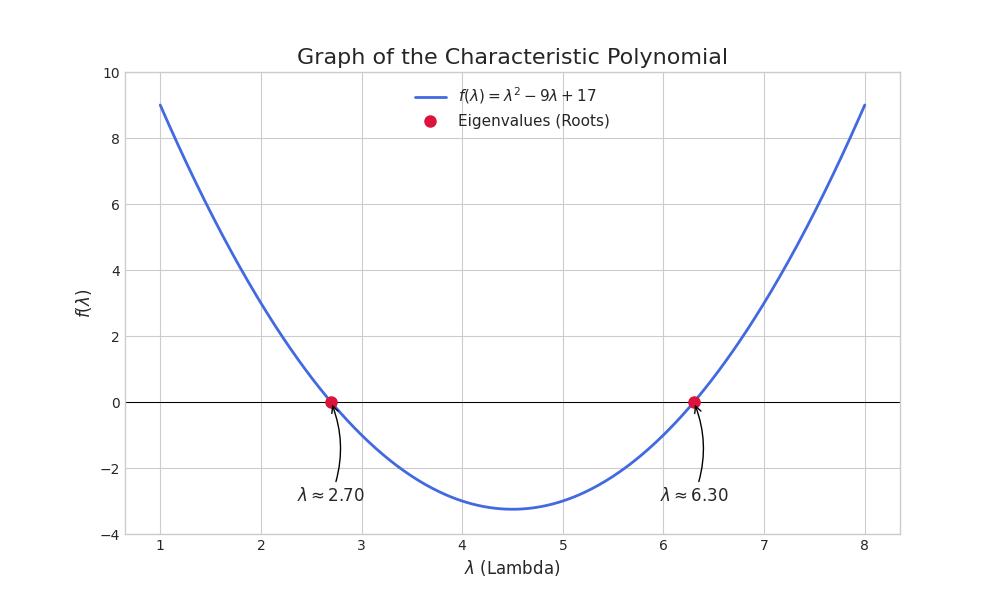
\includegraphics[width=0.75\columnwidth]{graph23.png}
    \caption{Plot}
    \label{fig:placeholder}
\end{figure}
\end{frame}

\end{document}